\documentclass[12pt, a4paper, final]{article}
%\documentclass[prodmode,acmtoms]{acmsmall}
\usepackage{amsmath,amstext,amsbsy,amsopn,amsthm,amscd,amsxtra,upref,amssymb}
\usepackage[dvips]{graphicx}
\usepackage{color}
\usepackage{algorithmic}
\usepackage{algorithm}
\usepackage{url}
\usepackage{fancybox}
%\pagestyle{empty}
%\newtheorem{thm}{Theorem}[subsection]
%\renewcommand{\thethm}{\arabic{subsection}.\arabic{thm}}
%\addtolength{\textwidth}{2cm}
%\addtolength{\voffset}{-2cm}
%\addtolength{\textheight}{3cm}
%\addtolength{\hoffset}{-3cm}
\setlength{\oddsidemargin}{0.25in}
\setlength{\textwidth}{6in}
\newtheorem{thm}{Theorem}
\newtheorem{lemma}{Lemma}
\newtheorem{theorem}{Theorem}
\newtheorem{corollary}{Corollary}
\newtheorem{proposition}[thm]{Proposition}
\newtheorem{example}[thm]{Example}
\newtheorem{remark}[thm]{Remark}
\newtheorem{discussion}[thm]{Discussion}
\newtheorem{definition}[thm]{Definition}
\newcommand{\Real}{\mathbb R}
\newcommand{\Cplx}{\mathbb C}
\newcommand{\Ker}{\operatorname{Ker}}
\newcommand{\Range}{\mathcal{R}}
\newcommand{\diag}{\operatorname{diag}}
%%\newcommand{\det}{\operatorname{det}}
\newcommand{\nice}[1]{\mathcal{#1}}
\newcommand{\slijedi}{\longrightarrow}
\newcommand{\kupa}[1]{\breve{#1}}
\newcommand{\todo}[1]{\textcolor{red}{#1}}
\newcommand{\eps}{\epsilon}
\newcommand{\tr}{*}
\newcommand{\cc}[1]{\overline{#1}}
\newcommand{\redvel}{\mathcal{O}}
\newcommand{\off}{\operatorname{off}}
\newcommand{\gap}{\operatorname{gap}}
\newcommand{\konv}[1]{\mathop{\longrightarrow}\limits^{#1}}
%%\newcommand{\imunit}{\mathfrak{i}}
\newcommand{\mm}[2]{{#1}^{(#2)}}
\newcommand{\ms}[2]{{#1}^{[#2]}}
\newcommand{\msn}[2]{{\mathcal{#1}}^{[#2]}}
\newcommand{\m}[2]{{\mathcal{#1}}^{(#2)}}
\newcommand{\mn}[1]{{\mathcal{#1}}}
\newcommand{\QED}{$\blacksquare\checkmark$}
\newcommand{\mb}[1]{\left(\begin{array}{#1}}
\newcommand{\me}{\end{array}\right)}
\newcommand{\eqb}{\begin{equation}}
\newcommand{\eqe}{\end{equation}}
\newcommand{\eqab}{\begin{eqnarray}}
\newcommand{\eqae}{\end{eqnarray}}

\newcommand{\bfmu}{{\boldsymbol\mu}}
\newcommand{\bfsigma}{{\boldsymbol\sigma}}
\newcommand{\bfSigma}{{\boldsymbol\Sigma}}
\newcommand{\bflambda}{{\boldsymbol\lambda}}
\newcommand{\bfzeta}{{\boldsymbol\zeta}}
%%%%%%%%%%%%% added by Z.D.
\newcommand{\bfvareps}{{\boldsymbol\varepsilon}}
\newcommand{\bfeps}{{\boldsymbol\epsilon}}
\newcommand{\bfi}{{\boldsymbol i}}
\def\roff  {\mbox{\boldmath$\varepsilon$}}
\newcommand{\imunit}{\mathfrak{i}}
\newcommand{\RE}{\operatorname{Re}}
\newcommand{\IM}{\operatorname{Im}}
\newcommand{\SPEC}{\mathfrak{S}}
%%%%%%%%%%%%%

\numberwithin{equation}{section}
\renewcommand{\theequation}{\thesection.\arabic{equation}}
\title{\texttt{xGESVDQ}: A QR--preconditioned QR  method for computing the singular value decomposition \\ \emph{Installation and Testing} \\  \emph{User Guide}}

\author{Zlatko  Drma\v{c}\thanks{The author's work is supported by the Croatian Science Foundation, under
		grant HRZZ--IP-11-2013-9345.} \\ Department of Mathematics, Faculty of Science, University of Zagreb}

\begin{document}
\maketitle
%\tableofcontents
\begin{abstract}
	\texttt{xGESVDQ} \cite{drm-xgesvd-paper} is a LAPACK--based software for computing the
	singular value decomposition (SVD) by a preconditioned QR method. With respect to numerical accuracy, it is superior to the existing implementation of the QR method (\texttt{xGESVD}), and to the divide and conquer method (\texttt{xGESDD}) from LAPACK \cite{LAPACK}.
	Although it is theoretically not yet entirely understood, based on overwhelming numerical evidence, the new method can be considered almost as accurate as the Jacobi SVD \cite{dem-ves-92}, \cite{drm-ves-VW-1, drm-ves-VW-2}. The software has a built in error estimate device and the result is accompanied with realistic error bounds for both the singular values and the singular vectors. Numerical experiments show close match between the measured and estimated errors, which behave as predicted by the perturbation theory: for a full column rank $A$, the relative errors in the computed singular values depend on the scaled condition number $\min_{D=diag}\kappa_2(A D)$, and the errors in the singular vectors, in addition, depend on the relative separations between the neighboring singular values.  At the same time,  the new implementation exploits highly optimized \texttt{xGESVD} in libraries such as the Intel's MKL and it can be considered as method of choice for fast and accurate SVD. 
	Simple modular structure of the new software allows straightforward conversion to a ScaLAPACK parallel implementation.
	
	This document describes the main properties, using and testing of the implementation of the \texttt{xGESVDQ} subroutines.
\end{abstract}


%%%%%%%%%%%%%%%%%%%%%%%%%%%%%%%%%%%%%%%%%%%%%%%%%%%%%%%%%%%%%%%%%%%%%%%%%%%%%%%% Introduction

\section{Introduction}\label{S=Introduction}
The SVD (Singular Value Decomposition) is one of the most important decompositions in matrix computations, with a variety of applications in sciences and engineering.
State of the art numerical software library LAPACK \cite{LAPACK} contains three different methods for computing the SVD of general matrices: 
\begin{itemize}
\item \texttt{xGESVD}, which reduces the matrix to bidiagonal form and then it deploys the zero shift bidiagonal QR SVD; 
\item \texttt{xGESDD}, which also uses the bidiagonal reduction, but the bidiagonal SVD is computed via the \emph{divide and conquer} scheme; 
\item \texttt{xGEJSV}, \texttt{xGESVJ} which are one-sided Jacobi SVD methods. 
\end{itemize}
Among them, \texttt{xGESDD} is the fastest and least accurate; \texttt{xGEJSV} and \texttt{xGESVJ} are the most accurate but the slowest, although \texttt{xGEJSV} in some implementations was able to outperform \texttt{xGESVD}.


\texttt{xGESVDQ}, described in this document, is an enhanced version of \texttt{xGESVD} -- at a price of an extra pivoted QR decomposition (e.g. \texttt{xGEQP3}), the existing QR SVD \texttt{xGESVD} becomes nearly as accurate as the Jacobi SVD.
The numerical details of the method are given in \cite{drm-xgesvd-paper}, and it is implemented in the SVD library \texttt{xGESVDQ} which  provides LAPACK-style FORTRAN codes for computing the SVD decomposition of general matrices in the four data types REAL (\texttt{SGESVDQ}), DOUBLE PRECISION (\texttt{DGESVDQ}), COMPLEX (\texttt{CGESVDQ}) and DOUBLE COMPLEX (\texttt{ZGESVDQ}).
\\ 
 
\noindent In \S \ref{S=1} we give the necessary details for using the subroutines, and \S \ref{S=test} describes installation and testing.


\section{Calling \texttt{xGESVDQ}}\label{S=1}
The calling sequence of \texttt{xGESVDQ} follows the one of \texttt{XGESVD}, with few differences that reflect the specific new features of \texttt{xGESVDQ}.   
For the sake of brevity, we describe the arguments of \texttt{CGESVDQ} only. For the other three data types, the calling sequences are obtained \emph{mutatis mutandis} and will be clear from the comments in the source codes.
\subsection{Method and notation}
For simpler and more precise description of the code, in  Algorithm \ref{zd:ALG:eig:xgesvdq} we first describe the structure of the method.
On input, the (real or complex) matrix $A$ is assumed $m\times n$ with 
$m\geq n$. In applications with $m<n$, the usage of SVD should be
reformulated in terms of $A^*$, in the obvious way. 
%The implemented method computes a pivoted QR factorization
%\begin{equation}\label{eq:RRQR}
%\Pi_r A \Pi_c = Q \begin{pmatrix} R \cr 0 \end{pmatrix},\;\;Q^* Q = QQ^* = I_m,\;\;R=\left(\begin{smallmatrix} r_{11} & \cdots & r_{1n} \cr  & \ddots & \vdots \cr  &  & r_{nn}\end{smallmatrix}\right) ,
%\end{equation}
\begin{algorithm}[hbt]
	\caption{$(U, \Sigma, V) = \mbox{\texttt{xGESVDQ}}(A,\mbox{method})$ ($A\in\mathbb{C}^{m\times n}$, $m\geq n$)}
	\label{zd:ALG:eig:xgesvdq}
	\begin{algorithmic}[1]
		%\STATE \framebox{$(\lambda,U) = EIG(H)$}
		%
		\STATE $(\Pi_r A) \Pi_c = Q \begin{pmatrix} R \cr 0 \end{pmatrix}$ 
		
		\COMMENT{Initial row sorting by the permutation matrix $\Pi_r$ and QR factorization with
			dynamic column pivoting $\Pi_c$, e.g. \texttt{xGEQP3}, or simple pre-sorting.  Full pivoting is also an option.}
		%
		\STATE Determine the numerical rank $\rho$ of $R$ and set $R_\rho = R(1:\rho,1:n)$. 
		\IF{$\rho = n$ and condition estimate needed}
		%
		\STATE $\kappa\approx \|(R_\rho\mathrm{diag}(1/\|R_\rho(:,i)\|_2))^{-1}\|_2$  
		\COMMENT{Use e.g. \texttt{xPOCON} and adjust to the norm $\|\cdot\|_2$.}
		%
		\ENDIF
		\IF{method = "upper"}
		\STATE Compute the SVD $R_\rho = \widehat{U}\begin{pmatrix} \widehat{\Sigma}& 0_{\rho,n-\rho}\end{pmatrix}\widehat{V}^*$. \COMMENT{Use \texttt{xGESVD}}
		\STATE The SVD of $A$ is $A = U\Sigma V^* \equiv \left[\Pi_r^T Q \left(\begin{smallmatrix} \widehat{U} & 0 \cr 0 & I_{m-\rho}\end{smallmatrix}\right)\right] \left(\begin{smallmatrix} \widehat{\Sigma} & 0_{\rho,n-\rho} \cr 0_{m-\rho,\rho} & 0_{m-\rho,n-\rho}\end{smallmatrix}\right) (\Pi_c\widehat{V})^*$
		\ELSE
		\STATE Compute the SVD $R_\rho^* = \widehat{U}\left(\begin{smallmatrix}\widehat{\Sigma}\cr 0_{m-\rho,\rho}\end{smallmatrix}\right)\widehat{V}^*$. \COMMENT{Use \texttt{xGESVD}}
		\STATE The SVD of $A$ is $A = U\Sigma V^* \equiv \left[\Pi_r^T Q \left(\begin{smallmatrix} \widehat{V} & 0 \cr 0 & I_{m-\rho}\end{smallmatrix}\right)\right] \left(\begin{smallmatrix} \widehat{\Sigma} & 0_{\rho,n-\rho} \cr 0_{m-\rho,\rho} & 0_{m-\rho,n-\rho}\end{smallmatrix}\right) (\Pi_c\widehat{U})^*$
		\ENDIF 
		%
		%
	\end{algorithmic}
\end{algorithm}
\subsection{Argument list (\texttt{CGESVDQ})}
\begin{verbatim}
SUBROUTINE CGESVDQ( JOBA, JOBP, JOBR, JOBU, JOBV, m, n, A, LDA, S, U,
 LDU, V, LDV, NUMRANK, IWORK, CWORK, LCWORK, RWORK, LRWORK, INFO )
\end{verbatim}
\begin{itemize}
	\item[1.] \doublebox{\textbf{JOBA}} [\emph{input}][{\sc CHARACTER}] 
	
	Provides information on the level of accuracy expected for the SVD of $A$.
	It specifies the cutoff threshold for truncating the smallest rows of the computed upper triangular factor $R$, thus truncating the smallest singular values. (The index $k$ described below defines the value of $\rho$ in Line 2. in Algorithm \ref{zd:ALG:eig:xgesvdq}; $\roff$ is the roundoff unit.) 
	\begin{itemize}
		\item[\framebox{'A'}] This is the most aggressive option. After the initial QR factorization, the upper triangular factor will be truncated at the smallest index $k$ such that the truncated part $R(k+1:n,k+1:n)$ of $R$ is below $\roff \sqrt{n}\max_{i=1:n}\|A(:,i)\|_2$ ($\equiv \roff \sqrt{n} |R_{11}|$ in case of column pivoting that brings the largest column to the fore). In this case, the smallest $n-k$ singular values are flushed to zero, but the backward error is still within the standard backward stability parameters as in \texttt{xGESVD} and \texttt{xGESDD}.
		\item[\framebox{'M'}] Similar as in the previous case, but the cutoff criterion is milder. The truncation occurs at the smallest index $k$ for which $|R_{k+1,k+1}| \leq \roff |R_{kk}|$. 
		\item[\framebox{'H'}] High relative accuracy requested. A submatrix $R(k+1:n,k+1:n)$ will be truncated only if it is zero.
		\item[\framebox{'E'}] This is the expert level. The level of accuracy is the same as with 'H', and, in addition, information needed for error estimate in the computed singular values and vectors is provided. The relevant (scaled) condition number is estimated and returned in \textbf{RWORK}. If $R$ is computed as singular, the scaled condition number of its largest leading nonsingular submatrix will be estimated.
	\end{itemize}
	\item[2.] \doublebox{\textbf{JOBP}} [\emph{input}][{\sc CHARACTER}] 
	
	Specifies the pivoting in the initial QR factorization, i.e. it determines whether to use row pivoting. (Permutation matrix $\Pi_r$ in Line 1 of Algorithm \ref{zd:ALG:eig:xgesvdq}.)
	\begin{itemize}
		\item[\framebox{'P'}] Prior to the column pivoted QR factorization, the rows of $A$ are permuted by a permutation $\pi$ such that $$\|A(\pi(1),:)\|_\infty \geq \|A(\pi(2),:)\|_\infty\geq\cdots\geq \|A(\pi(m),:)\|_\infty .$$ For high accuracy, this option is recommended if it is expected that $A$ might have differently scaled rows, and high accuracy is desired.
		\item[\framebox{'N'}] No row pivoting is used. The QR factorization in Line 1. of Algorithm \ref{zd:ALG:eig:xgesvdq} is computed only with a rank revealing column pivoting.
	\end{itemize}
	\item[3.] \doublebox{\textbf{JOBR}} [\emph{input}][{\sc CHARACTER}]
	Specifies whether te SVD of $R$ or $R^*$ is computed. Both choices will work well numerically. This option is left for the implementor to decide which can be better optimized. Researchers can use this option for further study of the numerical properties of the bidiagonalization and the structure of the bidiagonal form. 
	\begin{itemize}
	\item[\framebox{'T'}] The SVD of $R^*$ is computed and used in assembling the SVD of $A$.    
		\item[\framebox{'N'}] The SVD of $R$ is computed and used in assembling the SVD of $A$. This may be preferred as it involves less data movement (matrix transpositions).  
	\end{itemize}
	\item[4.] \doublebox{\textbf{JOBU}} [\emph{input}][{\sc CHARACTER}]
	\begin{itemize}
		\item[\framebox{'A'}] All $m$ left singular vectors are computed and returned as columns in the array $\mathbf{[U]}$. See the description of $\mathbf{[U]}$.
		\item[\framebox{'S'}] or \framebox{'U'} The leading $n$ left singular vectors are computed and returned as the leading $n$ columns in the array $\mathbf{[U]}$. See the description of $\mathbf{[U]}$.
		\item[\framebox{'R'}] The leading $r$ left singular vectors (belonging to the $r$ largest nonzero singular values) are computed and returned as columns in the array $\mathbf{[U]}$. Here $r=\mbox{\textbf{NUMRANK}}$ is the numerical rank that is determined by counting nonzero computed singular values. The value of $r$ can be smaller that $\rho$, determined after the first QR factorization (depending on \textbf{JOBA}). (\texttt{CGESVDQ} actually computes $\rho$ vectors, and $r<\rho$ may occur e.g. due to underflowed singular values.)
		\item[\framebox{'F'}] The $n$ left singular values are computed and returned in factored form as the product of the $Q$ factor from the initial QR factorization and the
		$n$ left singular vectors of $(R^* , 0)^*$. If row pivoting is used, then the necessary information on the row pivoting is stored in \textbf{IWORK}(N+1:N+M-1).	
		See the descriptions of $\mathbf{A}$, 
		$\mathbf{U}$, \textbf{CWORK}, \textbf{IWORK}.  See \S \ref{SSS=U=F}.
		\item[\framebox{'N'}] The left singular vectors are not computed. The array $\mathbf{[U]}$ is not referenced. 
	\end{itemize}
	
	\item[5.] \doublebox{\textbf{JOBV}} [\emph{input}][{\sc CHARACTER}]
	\begin{itemize}
		\item[\framebox{'A'}] or \framebox{'V'} All $n$ right singular vectors are computed and returned as conjugate transposed in the rows of the array $\mathbf{[V]}$.
		\item[\framebox{'R'}] The leading $r$ right singular vectors are computed and returned as conjugate transposed in te rows of the array $\textbf{[V]}$.  Here $r=\mbox{\textbf{NUMRANK}}$ is the numerical rank that is determined by counting nonzero computed singular values. The value of $r$ can be smaller that $\rho$, determined after the first QR factorization (depending on \textbf{JOBA}). (\texttt{CGESVDQ} actually computes $\rho$ vectors.)
		This option is allowed only if the same is set for \textbf{JOBU}, or if \textbf{JOBU}='N'. Otherwise, illegal value is declared.
		\item[\framebox{'N'}] The right singular vectors are not computed. If \textbf{JOBA}='E', the array $\mathbf{[V]}$ might be used as a workspace; see the description of $\mathbf{[V]}$.
	\end{itemize}
	
	\item[6.] \doublebox{{$\mathbf{m}$}} [\emph{input}][{\sc INTEGER}]
	
	The number of rows of the matrix; $m\geq 0$.
	
	\item[7.] \doublebox{{$\mathbf{n}$}} [\emph{input}][{\sc INTEGER}]
	
	The number of columns of the matrix; $0\leq n \leq m$.
	
	\item[8.] \doublebox{{$\mathbf{A}$}} [\emph{input/workspace/output}][{\sc COMPLEX ARRAY}][\textbf{LDA} $\times \mathbf{n}$]
	
	On input, $\mathbf{[A]}$ contains the matrix $A$. After the QR factorization, the part of $\mathbf{[A]}$ below the main diagonal contains the Householder vectors used in the factorization. If \textbf{JOBU} $\neq$ 'N', that part of $\mathbf{[A]}$ is left unchanged on the output. If \textbf{JOBU} = 'F', it will be used to restore or to apply the matrix of the left singular vectors.
	
	\item[9.] \doublebox{\textbf{LDA}} [\emph{input}][{\sc INTEGER}]
	
	The leading dimension of the array $\mathbf{[A]}$.  \textbf{LDA}$\geq\max(1,\mathbf{m})$.
	
	\item[10.] \doublebox{{$\mathbf{S}$}} [\emph{output}][{\sc REAL ARRAY}][$\mathbf{n}\times 1$]
	
	The computed singular values of $A$, ordered so that
	
	 $\mathbf{S}(i)\geq \mathbf{S}(i+1)$, $i=1,\ldots, \mathbf{n}-1$.
	
	\item[11.] \doublebox{{$\mathbf{U}$}} [\emph{output}]
	[{\sc COMPLEX ARRAY}] The dimensions of $\mathbf{[U]}$ are determined as follows:
	\begin{itemize}
		\item[(i)] \framebox{\textbf{LDU}$\times\mathbf{m}$}, if \textbf{JOBU} = 'A'; see the description of \textbf{LDU}. In this case, on exit, $\mathbf{[U]}$ contains the $\mathbf{m}$ left singular vectors.
		\item[(ii)] \framebox{\textbf{LDU}$\times\mathbf{n}$}, if \textbf{JOBU} $\in\{\mbox{'S', 'U', 'R'}\}$ ; see the description of \textbf{LDU}. In this   case, $\mathbf{[U]}$ contains the leading $\mathbf{n}$ or the leading $r$ left singular vectors, where $r=\mbox{\textbf{NUMRANK}}$ is the numerical rank. See the description of \textbf{JOBU}.
		\item[(iii)] \framebox{\textbf{LDU}$\times\mathbf{n}$}, if \textbf{JOBU} = 'F' ; see the description of \textbf{LDU}. In this case $\mathbf{[U]}$   contains the $n\times n$ matrix of the left singular vectors of the upper triangular matrix $R$ from Line 1. of Algorithm \ref{zd:ALG:eig:xgesvdq}. This information can be used to form the left singular vectors of $\mathbf{A}$.
	\end{itemize}
	If \textbf{JOBU} = 'N', then $\mathbf{[U]}$ is not referenced. 
	
	\item[12.]  \doublebox{\textbf{LDU}} [\emph{input}][{\sc INTEGER}]
	
	The leading dimension of the array $\mathbf{[U]}$.
	\begin{itemize}  
		\item[(i)]  If \textbf{JOBU} $\in\{\mbox{'A', 'S', 'U', 'R'}\}$, then  \textbf{LDU}$\geq \max(1,\mathbf{m})$.  
		\item[(ii)]  If \textbf{JOBU} = 'F',  then \textbf{LDU}$\geq \max(1,\mathbf{n})$.
		\item[(iii)]  Otherwise, \textbf{LDU} $\geq 1$.
	\end{itemize}
	
	\item[13.]  \doublebox{{$\mathbf{V}$}} [\emph{workspace/output}]  [{\sc COMPLEX ARRAY}] The dimensions of $\mathbf{[V]}$ are determined as follows:
	\begin{itemize}
		% \item  \textbf{LDV}$\times\mathbf{n}$ if \textbf{JOBV} $\in\{\mbox{'A', 'V', 'R'}\}$, or if \textbf{JOBA} = 'E' .
		\item[(i)]  \textbf{LDV}$\times\mathbf{n}$, if \textbf{JOBV} = 'A', or 'V'. In that case  $\mathbf{[V]}$ contains the $\mathbf{n}\times\mathbf{n}$ unitary matrix $V^*$; if \textbf{JOBA} = 'E', it is also used as a workspace.
		\item[(ii)]  \textbf{LDV}$\times\mathbf{n}$, if \textbf{JOBV} = 'R'. In that case  $\mathbf{[V]}$ contains the first $r=\mbox{\textbf{NUMRANK}}$ rows of $V^*$ (the right singular vectors, stored rowwise, of the \textbf{NUMRANK} largest singular values).
		If \textbf{JOBA} = 'E', it is also used as a workspace.
		\item[(iii)]  If \textbf{JOBV} ='N' and \textbf{JOBA} = 'E', $\mathbf{[V]}$ is used only as a workspace.  
	\end{itemize}
	If \textbf{JOBV} = 'N', and \textbf{JOBA}$\neq$'E', $\mathbf{[V]}$ is not referenced. 
	%%%%%%%%%%%%%%%%%%%%%%%%%%%%%%%%%%%%%%%%%%%%%%%%%%%%%%%%%%%%%%%%%%
	\item[14.] \doublebox{\textbf{LDV}} [\emph{input}][{\sc INTEGER}]
	
	The leading dimension of the array $\mathbf{[V]}$. 
	\begin{itemize} 
		\item[(i)] If \textbf{JOBV} $\in\{\mbox{'A', 'V', 'R'}\}$  or \textbf{JOBA} = 'E', then \textbf{LDV} $\geq\max(\mathbf{n},1)$.  
		\item[(ii)] Otherwise, \textbf{LDV} $\geq 1$.     
	\end{itemize} 
	%%%%%%%%%%%%%%%%%%%%%%%%%%%%%%%%%%%%%%%%%%%%%%%%%%%%%%%%%%%%%%%%%%%
	\item[15.] \doublebox{\textbf{NUMRANK}} [\emph{output}][{\sc INTEGER}]
	
	\textbf{NUMRANK} is first set to the numerical rank determined after the rank revealing QR factorization, following the strategy determined by te value of \textbf{JOBA}. If \textbf{JOBV}='R', and if \textbf{JOBU}='R', only \textbf{NUMRANK} leading singular values and vectors are then requested in the call of \texttt{CGESVD}. The value of  \textbf{NUMRANK} might be further reduced if some smallest singular values of the triangular factor are computed by \texttt{CGESVD} as exact zeros. (This is possible, e.g. due to underflows.)
	%%%%%%%%%%%%%%%%%%%%%%%%%%%%%%%%%%%%%%%%%%%%%%%%%%%%%%%%%%%%%%%%%%%%
	\item[16.] \doublebox{\textbf{IWORK}} [\emph{workspace/output}][{\sc INTEGER ARRAY}]
	The length of \textbf{IWORK} is:
	\begin{itemize}
		\item[(i)] \framebox{$\mathbf{n} + \mathbf{m} - 1$},  if \textbf{JOBP} = 'P', 
		\item[(ii)] \framebox{$\mathbf{n}$}, \hspace{1.3cm} if \textbf{JOBP} = 'N'
	\end{itemize} 
	On exit, \textbf{IWORK}$(1:\mathbf{n})$ contains column pivoting permutation of the rank revealing QR factorization.
	If \textbf{JOBP} = 'P', \textbf{IWORK}$(\mathbf{n}+1:\mathbf{n}+\mathbf{m}-1)$ contains the indices of the sequence of row swaps used in row pivoting. These can be used to restore the left singular vectors in the case \textbf{JOBU}='F'. See \S \ref{SSS=U=F}.
	
	\underline{\textbf{Note:}} In case of real data type (\texttt{SGESVDQ}, \texttt{DGESVDQ}) the length of \textbf{IWORK} increases by $\mathbf{n}$ in both cases above if \textbf{JOBA}='E'.
	%%%%%%%%%%%%%%%%%%%%%%%%%%%%%%%%%%%%%%%%%%%%%%%%%%%%%%%%%%%%%%%%%%%
	\item[17.] \doublebox{\textbf{CWORK}} [\emph{workspace/output}][{\sc COMPLEX ARRAY}][\textbf{LCWORK}$\times 1$]
	\begin{itemize}
		\item[(i)] If, on entry, \textbf{LCWORK} $\neq -1$, then on exit \textbf{CWORK}$(1:\mathbf{n})$ contains parameters needed to recover the $Q$ factor from the QR factorization computed by \texttt{CGEQP3}.
		
		\item[(ii)] If, on entry, \textbf{LCWORK} = -1, then a workspace query is assumed and \textbf{CWORK} must be of length at least two.
		On exit \textbf{CWORK}(1) contains the optimal length of \textbf{CWORK} and \textbf{CWORK}(2) contains the minimal length.
	\end{itemize}
	%%%%%%%%%%%%%%%%%%%%%%%%%%%%%%%%%%%%%%%%%%%%%%%%%%%%%%%%%%%%%%%%%
	\item[18.] \doublebox{\textbf{LCWORK}} [\emph{input/output}][{\sc INTEGER}]
	
	The dimension of the array \textbf{CWORK}. 
	\begin{itemize}
		\item[(i)] If, on entry, \textbf{LCWORK} $=-1$, (workspace query) then the optimal and the minimal length of \textbf{CWORK} are computed and returned in the first two entries of \textbf{CWORK}. 
		%See the description of \textbf{CWORK}. 
		
		\item[(ii)] Otherwise, on entry, \textbf{LCWORK} must contain the length of \textbf{CWORK}. This ensures that the work space of proper length is allocated. The minimal and the maximal requirements depend on the workspaces required for \texttt{CGEQP3}, \texttt{CGESVD} and \texttt{CUNMQR} and are determined as follows:
		For the minimal length, define 
		\begin{itemize}
			\item[] LWQP3\ \ \ \ = $\mathbf{n}+1$ (minimal workspace length for $\mathbf{m}\times \mathbf{n}$ \texttt{CGEQP3}),\footnote{In case of real data type, LWQP3 = $3\mathbf{n}+1$.}  
			\item[] LWUNQ \ \ = (minimal workspace length for 'left' $\mathbf{m}\times\mathbf{n}$ \texttt{CUNMQR}) = 
			\begin{itemize}\item[] 1. $\max(\mathbf{n},1)$ if \textbf{JOBU} ='R', 'S', or 'U' ; \item[] 2. $\max(\mathbf{m},1)$ if \textbf{JOBU} ='A' \end{itemize}
			\item[]  LWSVD \ \ \ = $\max(1,3 \mathbf{n})$ (minimal workspace length for $\mathbf{n}\times \mathbf{n}$ \texttt{CGESVD})\footnote{In case of real data type, LWSVD = $5\mathbf{n}$.}
			\item[]  LWSVD2 \ = $\max(1,3 (\mathbf{n}/2))$ (minimal workspace length for $\mathbf{n}/2\times \mathbf{n}/2$ \texttt{CGESVD})
			\item[] LWLQF \ \ \ = $\max(1,\mathbf{n}/2)$ (minimal workspace length for $\mathbf{n}/2 \times \mathbf{n}$ \texttt{CGELQF})
			\item[] LWQRF \ \ \ = $\max(1,\mathbf{n}/2)$ (minimal workspace length for $\mathbf{n} \times \mathbf{n}/2$ \texttt{CGEQRF})
			\item[] LWUNLQ  = $\max(1,\mathbf{n})$ (minimal workspace length for 'right' $\mathbf{n} \times \mathbf{n}$ \texttt{CUNMLQ})
			\item[] LWUNQ2  = $\max(1,\mathbf{n})$ (minimal workspace length for 'right' $\mathbf{n} \times \mathbf{n}$ \texttt{CUNMLQ})
			\item[] LWCON \ \  = $2 \mathbf{n}$ (minimal workspace length for  $\mathbf{n} \times \mathbf{n}$ \texttt{CPOCON})\footnote{In case of real data type, LWCON = $3\mathbf{n}$.}
			%\begin{itemize}
			%	\item[]\hspace{1.2cm} $= 3 \mathbf{n}$, if the left singular vectors are not requested
			% 	\item[]\hspace{1.2cm} $= 2\mathbf{n}+\mathbf{m}$, if the left singular vectors are requested 
			% 	\end{itemize}
		\end{itemize}
		Then the minimal value of \textbf{LCWORK} is:
		\begin{itemize} 	     
			\item[\framebox{$\Sigma$}] \begin{itemize} \item[$\circ$] $\max( \mathbf{n} + \mbox{LWQP3}, \mbox{LWSVD} )$, if only the singular values are needed;
				\item[$\bullet$] $\max( \mathbf{n} + \mbox{LWQP3}, \mbox{LWCON}, \mbox{LWSVD})$, if the singular values and a scaled condition estimate are requested;
			\end{itemize}
			\item[\framebox{$\Sigma, U$}] \begin{itemize}\item[$\circ$] $\mathbf{n} + \max( \mbox{LWQP3}, \mbox{LWSVD}, \mbox{LWUNQ} )$, if the singular values and the left  singular vectors are requested;
				\item[$\bullet$] $\mathbf{n} + \max( \mbox{LWQP3}, \mbox{LWCON}, \mbox{LWSVD}, \mbox{LWUNQ} )$, if the singular values, the left  singular vectors and a scaled condition estimate are requested;
			\end{itemize}	
			\item[\framebox{$\Sigma, V$}] \begin{itemize}\item[$\circ$] $\mathbf{n} + \max( \mbox{LWQP3}, \mbox{LWSVD} )$,  if the singular values and the right
				singular vectors are requested;
				\item[$\bullet$] $\mathbf{n} + \max( \mbox{LWQP3}, \mbox{LWCON}, \mbox{LWSVD} )$,  if the singular values, the right
				singular vectors and a scaled condition estimate are requested; 
			\end{itemize}
			\item[\framebox{$\Sigma, U, V$}] \begin{itemize} \item[$\circ$] $\mathbf{n} + \max( \mbox{LWQP3}, \mbox{LWSVD}, \mbox{LWUNQ} )$, if the full SVD is requested, \textbf{JOBV}='R', and independent of \textbf{JOBR};
				\item[$\bullet$] $\mathbf{n} + \max( \mbox{LWQP3}, \mbox{LWCON}, \mbox{LWSVD}, \mbox{LWUNQ} )$, if the full SVD with scaled condition estimate is requested, \textbf{JOBV}='R', and independent of \textbf{JOBR}.	
			\end{itemize}
			The above specified length of \textbf{CWORK} suffices also if \textbf{JOBV}='A' and the numerical rank of $A$ (as seen after the rank revealing QR factorization) is at least $\mathbf{n}/2$. However, if \textbf{JOBV}='A' and $A$ is estimated of low numerical rank, then a more efficient computation is possible and in that case the length of work is determined as follows:
			\begin{itemize}
				\item[$\lozenge$] $\max($ $\mathbf{n} + \max( \mbox{LWQP3}$, $\mbox{LWSVD}$, $\mbox{LWUNQ})$, $\mathbf{n} + \max( \mbox{LWQP3}, \mathbf{n}/2+\mbox{LWLQF}, \mathbf{n}/2+\mbox{LWSVD2}, \mathbf{n}/2+\mbox{LWUNLQ}, \mbox{LWUNQ}) )$ if the  
				full SVD is requested with \textbf{JOBV}='A', 'V', and \textbf{JOBR} ='N' ;
				\item[$\blacklozenge$]	 $\max(\mathbf{n} + \max( \mbox{LWQP3}, \mbox{LWCON}, \mbox{LWSVD}, \mbox{LWUNQ})$, $\mathbf{n} + \max( \mbox{LWQP3}$, $\mbox{LWCON}, \mathbf{n}/2+\mbox{LWLQF}, \mathbf{n}/2+\mbox{LWSVD2}, \mathbf{n}/2+\mbox{LWUNLQ}, \mbox{LWUNQ}) )$ if the  
				full SVD with scaled condition estimate is requested, with \textbf{JOBV}='A', 'V', and \textbf{JOBR} ='N' ;
				\item[$\vartriangle$] $\max( \mathbf{n} + \max( \mbox{LWQP3}, \mbox{LWSVD}, \mbox{LWUNQ} )$, $\mathbf{n} + \max( \mbox{LWQP3}, \mathbf{n}/2+\mbox{LWQRF}$, $\mathbf{n}/2+\mbox{LWSVD2}, \mathbf{n}/2+\mbox{LWUNQ2}, \mbox{LWUNQ} ) )$ if the
				full SVD is requested with \textbf{JOBV}='A', 'V', and \textbf{JOBR} ='T';
				\item[$\blacktriangle$] $\max( \mathbf{n} + \max( \mbox{LWQP3}, \mbox{LWCON}$, $\mbox{LWSVD}, \mbox{LWUNQ} )$, $\mathbf{n} + \max( \mbox{LWQP3}$, $\mbox{LWCON}$, $\mathbf{n}/2+\mbox{LWQRF}$, $\mathbf{n}/2+\mbox{LWSVD2}, \mathbf{n}/2+\mbox{LWUNQ2}, \mbox{LWUNQ} ) )$ if the
				full SVD with scaled condition estimate is requested with \textbf{JOBV}='A', 'V', and \textbf{JOBR} ='T';
			\end{itemize}
		\end{itemize} 	
		The optimal value of \textbf{LCWORK} is determined analogously, using the optimal workspace lengths for \texttt{CGEQP3}, \texttt{CGESVD} and \texttt{CUNMQR}.
	\end{itemize}	
	
	% 		*...
	\item[19.] \doublebox{\textbf{RWORK}} [\emph{workspace/output}][{\sc REAL ARRAY}][\textbf{LRWORK}$\times 1$]
	
	On exit, if \textbf{JOBA}='E', \textbf{RWORK}(1) contains an estimate  of $\sqrt{\|(A_c^* A_c)^{-1}\|_1}$, where $A_c$ is obtained from $A$ by normalizing its columns to unit Euclidean length. Otherwise, 
	\textbf{RWORK}(1)= -1. See \S \ref{SSS=condest}.
	
	\textbf{RWORK}(2) contains the number of singular values computed as exact zeros when \texttt{CGESVD} is applied to the (possibly truncated) matrix $R$. See the description of \textbf{NUMRANK}.
	
	In case of early exit (no call to \texttt{CGESVD}, such as in the case of zero matrix) \textbf{RWORK}(2)=-1.
	
	\item[20.] \doublebox{\textbf{LRWORK}} [\emph{input}][{\sc INTEGER}]
	
	The dimension of the array \textbf{RWORK}.
	If \textbf{JOBP}='P', then {\textbf{LRWORK} $\geq \max(2, \mathbf{m}, 5\mathbf{n})$}. Otherwise, {\textbf{LRWORK} $\geq \max(2, 5\mathbf{n})$}.
	\item[21.]  \doublebox{\textbf{INFO}} [\emph{output}][{\sc INTEGER}]
	\begin{itemize}
		\item[\framebox{$=0$}]:  successful exit.
		\item[\framebox{$<0$}]:  if \textbf{INFO} = $-i$, the $i$-th argument had an illegal value.
		\item[\framebox{$>0$}]:  if \texttt{CBDSQR} did not converge, \textbf{INFO} specifies how many superdiagonals of an intermediate bidiagonal form $B$ (computed in \texttt{CGESVD}) did not converge to zero.
	\end{itemize}
\end{itemize}

\subsection{Further details}

\subsubsection{Using the condition number estimate for error bounds}\label{SSS=condest}
Since the method first computes the triangular factor $R$, the condition number that gives a realistic error bound in most cases can be efficiently estimated as follows: 
The columns of the upper triangular factor $R$ are scaled to have unit Euclidean norms; the scaled matrix is denoted by $R_c$. 
If $A_c$ is defined analogously, then $\Pi_c^T A_c^* A_c\Pi_c=R_c^* R_c$.
Then, assuming full rank of $A$, \texttt{xPOCON} is used to estimate $\|(R_c^* R_c)^{-1}\|_1$( $=\|(A_c^* A_c)^{-1}\|_1$), and
finally we deploy the relations	
$$
n^{-1/4} \sqrt{\|(A_c^* A_c)^{-1}\|_1} \leq \|A_c^{\dagger}\|_2 \leq n^{1/4} \sqrt{\|(A_c^* A_c)^{-1}\|_1},
$$
that can be easily proved using the properties of the matrix norms.
Since $1\leq \|A_c\|_2\leq \sqrt{n}$, $\kappa_2(A_c)\equiv \|A_c\|_2\|A_c^{\dagger}\|_2\leq n^{3/4}\sqrt{\|(A_c^* A_c)^{-1}\|_1}$.
Then, the error bounds for the computed singular values and vectors are
derived as explained in \cite{drm-xgesvd-paper}. One should be careful when the estimated scaled condition number exceeds the inverse of the machine precision, because in such cases it might be a considerable underestimate of the true value.
% $\kappa_{scaled}(A)$.
\subsubsection{Using left singular vectors in factored form}\label{SSS=U=F}
The option to leave the left singular vectors in factored form is useful in the case of tall and skinny $A$ ($m\gg n$) that is e.g. the coefficient matrix in a least square problem $\|Ax-b \|_2\rightarrow\min$, solved by SVD. The unique minimum norm optimal $x$ is given as $x=A^{\dagger}b\equiv V\Sigma^{\dagger}U^* b$. Note that in that case the computation of $U^* b$ reads (see e.g. line 8 in Algorithm \ref{zd:ALG:eig:xgesvdq}; similarly with the data given in line 11)
$$
b \leftarrow  \left( \begin{smallmatrix} \widehat{U}^* & 0 \cr 0 & I_{m-\rho}\end{smallmatrix}\right)( Q^* (\Pi_r b) ) 
$$
and it is easily implemented using \texttt{CLASWP}, \texttt{CUNMQR} and \texttt{CGEMM}. Of course, if one wants to form $U$ explicitly,
the matrix $\widehat{U}$ should be placed in the leading block of the
array $U$ that is initialized as $n$ columns of the identity $I_m$, and $U$ should be pre-multiplied by $Q$ using
\texttt{CUNMQR}. For instance, the first $n$ left singular vectors are recovered by the following code:
%If one wants $U$ explicitly formed, on exit from \texttt{CGESVDQ}, the following code will do the job:
\begin{verbatim}
CALL CUNMQR( 'Left', 'No_Tr', m, n, n, A, LDA, CWORK, U, LDU,  &
CWORK(N+1), LCWORK-N, IERR )  
IF ( ROWPRM ) CALL CLASWP( N1, U, LDU, 1, M-1, IWORK(N+1), -1 )
\end{verbatim}
The details can be seen in the source code of \texttt{xGESVDQ}.
%\subsection{Notes to a implementor}
\subsubsection{Linker information}
\texttt{xGESVDQ} subroutines are built on top of BLAS and LAPACK computational and driver subroutines. 
\subsubsection{Updates and maintenance}
\texttt{xGESVDQ} subroutines are designed in the LAPACK environment
both as ready to use numerically sound software and as a developer's framework for accurate SVD computations. The two main ingredients are \texttt{xGEQP3} and \texttt{xGESVD}, and any future improvements and updates of these two subroutines are automatically incorporated in \texttt{xGESVDQ}. 
\subsubsection{Modifications and further research and development} The Businger-Golub column pivoting can be replaced with simple pre-sorting of the columns of $A$ with respect to their Euclidean lengths. This is implemented in the module \texttt{xGESVDQS} with simple replacement of the rank revealing QR factorization
\begin{verbatim}
CALL xGEQP3( M, N, A, LDA, IWORK, WORK, WORK(N+1), LWORK-N, IERR )
\end{verbatim}
with initial column sorting (encoded in the permutation vector \texttt{IWORK}) followed by the ordinary QR factorization,
\begin{verbatim}
CALL xLAPMT( .TRUE., M, N, A, LDA, IWORK )
CALL xGEQRF( M, N, A, LDA, WORK, WORK(N+1), LWORK-N, IERR )
\end{verbatim}
However since this static pre-sorting is not rank revealing, the options in \textbf{JOBA} are reduced to computation without ('H', without any intervention in the upper tringular factor $R$) or with scaled condition number estimatation ('E') in the case of full rank $R$. For details see \cite{drm-xgesvd-paper}.  The module \texttt{xGESVDQS} is not included in this distribution, and it is available, upon request, from the author.  

Another option is to use the windowed pivoting \texttt{xGEQPX}, \texttt{xGEQPY} from
\cite{bischof-q-orti-RRQR-1998}, \cite{bischof-q-orti-RRQR-1998-TOMS782}. We omit the details fo the sake of brevity, and refer to \cite{drm-xgesvd-paper}.

Further, one could replace e.g. \texttt{xGESVD} with some other SVD algorithm such as \texttt{xGESDD}, but in that case we do not expect as dramatic improvement in accuracy because the bidiagonal divide an conquer algorithm in \texttt{xGESDD} is not as accurate as the zero shift bidiagonal QR SVD. In other words, in this framework \texttt{xGESVD} can be turned into a highly accurate procedure that delivers both accurate output (when warranted bu the data) and a reliable error bound, and \texttt{xGESDD} cannot. It remains to be explored how this applies to the fast bidiagonal SVD \cite{Grosser-Lang-2003}.

Future research will include studying whether and to what extent the bidiagonalization can benefit (in the sense of enhanced accuracy) from the communication avoiding tournament pivoting \cite{Demmel-CARRQR-15}.
%This would then open an interesting opportunity for a development of an accurate parallel QR SVD. 


\section{\texttt{xGESVDQ} test drivers: user guide}\label{S=test}

%\subsection{Technical background (\cite{drm-xgesvd-paper}, \cite{drm-xgesvd-short})}
%\texttt{xGESVDQ} is a LAPACK--based software for computing the
%singular value decomposition (SVD) by a preconditioned QR method. With respect to numerical accuracy, it is superior to the existing implementation of the QR method (\texttt{xGESVD} in LAPACK), and to the divide and conquer method (\texttt{xGESDD}).
%Although it is theoretically not yet entirely understood, based on overwhelming numerical evidence, the new method can be considered almost as accurate as the Jacobi SVD. The software has a built in error estimate device and the result is accompanied with realistic error bounds for both the singular values and the singular vectors. Numerical experiments show close match between the measured and estimated errors, which behave as predicted by the perturbation theory: for a full column rank $A$, the relative errors in the computed singular values depend on the scaled condition number $\min_{D=diag}\kappa_2(A D)$, and the errors in the singular vectors, in addition, depend on the relative separations between the neighboring singular values.  At the same time,  the new implementation exploits highly optimized \texttt{xGESVD} in libraries such as the Intel's MKL and it can be considered as method of choice for fast and accurate SVD. 
%Simple modular structure of the new software allows straightforward conversion to a ScaLAPACK parallel implementation.

\subsection{Directories and files}\label{SS=DIF}

In the \textbf{HOME} directory of the testing package, the program files
are organized in the subdirectories as follows:
\begin{itemize}
\item \textbf{HOME} 
\begin{itemize}
\item \textbf{xGESVDQ}
\item \textbf{REFVAL}
\item \textbf{MATGEN}
\item \textbf{TESTING}
\item \textbf{AUXSBR}	
\end{itemize}	
\end{itemize}
\subsubsection{xGESVDQ}
\textbf{xGESVDQ}  contains the source codes of the new SVD
algorithm in 4 data types
\begin{itemize}
\item \texttt{SGESVDQ.f} (single precision)
\item \texttt{DGESVDQ.f} (double precision)
\item \texttt{CGESVDQ.f} (complex)
\item \texttt{ZGESVDQ.f} (double complex)
\end{itemize}
These are the routine being tested. 
The routines are LAPACK-based and written in the LAPACK style. All four have been tested for compliance with FORTRAN standard, e.g. both
passed, without errors or warnings, \texttt{g77 -c -fpedantic *.f}, \texttt{g77 -c -fpedantic -ff90 *.f}

\noindent For theoretical background and  discussion of the numerical results, see \cite{drm-xgesvd-paper}.

\subsubsection{REFVAL}
\textbf{REFVAL}  contains simple one-sided
Jacobi SVD in double complex precision,
\begin{itemize}
\item \texttt{zgesvjx.f} (one sided double complex Jacobi SVD pure)
\end{itemize}
that is used for reference values in case of complex data.

\noindent For real test matrices (single and double precision), the reference values of the SVD are computed by double precision one sided Jacobi SVD \texttt{dgesvj()} from LAPACK. 

\subsubsection{MATGEN}
\textbf{MATGEN} contains the generators of test matrices
\begin{itemize}
\item \texttt{dmgen.f} (double precision)
\item \texttt{zmgen.f} (double complex)
\end{itemize}
See \cite[\S 3.1]{drm-xgesvd-paper} for more details on the kind of matrices
generated by these subroutines.

\subsubsection{TESTING}

\textbf{TESTING}  contains test drivers and makefiles

\begin{itemize}
\item \texttt{TestDGESVDQ.f} (interactive test for \texttt{SGESVDQ} and \texttt{DGESVDQ}; the user can choose different dimensions and options)
\item \texttt{TestDGESVDQ\_no\_input.f} (automatic test for \texttt{SGESVDQ} and \texttt{DGESVDQ}; the user can review the hard-coded test parameters and it is ony required to hit \framebox{\emph{enter}} to start the test)
\item \texttt{TestZGESVDQ.f} (interactive test for \texttt{CGESVDQ} and \texttt{ZGESVDQ}; the user can choose different dimensions and options)
\item \texttt{TestZGESVDQ\_no\_input.f} (automatic test for \texttt{CGESVDQ} and \texttt{ZGESVDQ}; the user can review the hard-coded test parameters and it is ony required to hit \framebox{\emph{enter}} to start the test)
\item \texttt{MakeTest} (make file for interactive test)
\item \texttt{MakeTest\_ni} (make file for automatic test with hard-coded parameters)
\end{itemize}

\noindent This directory also contains the Matlab script \texttt{TestSummary} that
can be used to display the test results in several figures, see \S \ref{EX}.

\subsubsection{AUXSBR}
\textbf{AUXSBR} contains auxiliary subroutines used by the test drivers:
\begin{itemize}
\item[--] for real data tests:

\begin{itemize}
\item[$\bullet$] \texttt{dchkor.f} (orthogonality check for singular vectors) 
\item[$\bullet$] \texttt{dcmpsv.f} (compares singular vectors with reference values)
\item[$\bullet$] \texttt{dresvd.f} (computed the residual norm for the SVD)   
\item[$\bullet$] \texttt{xges2d.f} (single to double precision matrix copy)
\item[$\bullet$] \texttt{xged2s.f} (double to single precision matrix copy)  
\end{itemize}

\item[--] for complex data tests:
\begin{itemize}
\item[$\bullet$] \texttt{zchkun.f} (orthogonality check for singular vectors) 
\item[$\bullet$] \texttt{zcmpsv.f} (compares singular vectors with reference values)
\item[$\bullet$] \texttt{zresvd.f} (computed the residual norm for the SVD)   
\item[$\bullet$] \texttt{xgec2z.f} (single complex to double complex precision matrix copy)
\item[$\bullet$] \texttt{xgez2c.f} (double complex to single complex precision matrix copy)
\end{itemize}
\end{itemize}

\subsection{Making the test driver executables}

\subsubsection{Linker information}
In addition to the files listed in \S \ref{SS=DIF}, the linker needs the BLAS ad LAPACK libraries. 
In the corresponding makefiles (\texttt{MakeTest}, \texttt{MakeTest\_ni}) the user should 
adjust the home page for the directories described in \S \ref{SS=DIF} and linker information
for BLAS and LAPACK. In the example files provided in this package
one can use sequential or threaded Intel MKL libraries.

\begin{itemize}
	\item interactive test drivers
\begin{itemize}
\item \texttt{make -f MakeTest rtestt}    (real data, threaded)
\item \texttt{make -f MakeTest rtests}   (real data, sequential)
\item \texttt{make -f MakeTest ctestt} (complex data, threaded)
\item \texttt{make -f MakeTest ctests} (complex data, sequential)
\end{itemize}
\item non-interactive test drivers; no input parameters 
\begin{itemize}
	\item \texttt{make -f MakeTest\_ni rtestt\_ni}    (real data, threaded)
	\item \texttt{make -f MakeTest\_ni rtests\_ni}   (real data, sequential)
	\item \texttt{make -f MakeTest\_ni ctestt\_ni} (complex data, threaded)
	\item \texttt{make -f MakeTest\_ni ctests\_ni} (complex data, sequential)
\end{itemize}
\end{itemize}
\subsection{Using the test drivers}
The test drivers can be used as interactive and automatic, with hard coded parameters. In either case, the run time can be considerable if the matrices are of larger dimensions. The total number of test cases in a single run is larger than 30000 and it can be larger than 60000. The purpose of the test is to determine to what extent the measured errors comply with the errors predicted by the perturbation theory.

\subsubsection{Detailed interactive test program}\label{SSS=ITP}

In a simple interactive menu, the test starts with choosing one of the following jobs

\begin{verbatim}
1. SIGMA only
2. SIGMA, U(MxN)
3. SIGMA, V(NxN)
4. SIGMA, U(MxN), V(NxN) 
5. SIGMA, U(MxM), V(NxN) 
6. SIGMA, U(MxM)
7. SIGMA, U(MxNR), V(NxNR), (here NR denotes the numerical rank)
8. SIGMA, V(NxNR)
9. SIGMA, U(NxNR)
\end{verbatim}

\noindent Next, accuracy level is set to one of the following:

\begin{verbatim}                         
(1) The requested accuracy corresponds to the backward
    error bounded by                                  
   || delta A ||_F <= f(m,n) * EPS * || A ||_F,       
    where EPS = {S,D}LAMCH(Epsilon). This authorises  
    {C,Z}GESVDQ to truncate the computed triangular   
    factor in the rank revealing QR factorization     
    whenever the truncated part is below the          
    threshold EPS * ||A||_F.                          
(2) Similarly as with (1), but the truncation is more 
    gentle: it is allowed only when there is a drop on
    the diagonal of the triangular factor.           
    This is a medium level of accuracy.               
(3) High accuracy requested. No numerical rank        
    determination based on the rank revealing QR      
    factorization is attempted.                       
(4) Accuracy level same as in (3), and in addition an  
    estimate of the scaled cond. number is computed.  
\end{verbatim}

\noindent Next, one can choose between only column or complete row and column pivoting. 

\begin{verbatim}
Select the pivoting in the initial QR factorization:
(1) Column-pivoted QR factorization as preconditioner.
(2) Row sorting prior to column pivoted QRF.
    (This may give more accurate results if the rows of A
    vary in length due to both ery large and very small
    weighting factors, causing large s_cond(A). 
\end{verbatim}

\noindent The computation of the SVD of $A$ proceeds with the SVD
of its computed triangular factor $R$. \texttt{xGESVDQ} can work
with both $R$ and $R^*$.

\begin{verbatim}
After the QR factorization, proceed with computing:
(1) The SVD of the upper triangular factor R 
    (This is recommended when using xGESVDQ.)
(2) The SVD of the conjugate-transposed R**H 
    (This involves more data movement and it is left
    as optional for experimenting in the R&D.)
\end{verbatim}

\noindent Finally, the row dimension $m$ and te column dimension $n$ are entered, and the number of test cases ($1$ or $2$) per class of test matrices is set.

\subsubsection{Example driver, no input required}

In this case, the options described in \S \ref{SSS=ITP} are hard-coded;
the user can review them and hit \framebox{\emph{enter}} to start the test.

\subsection{Visualization of the test results - one graph is worth thousands of numbers}
For the selected options, the test driver runs $32448$ or $64896$ test cases. The results of testing \texttt{xGESVDQ} are stored in the files
\begin{itemize}
\item \texttt{SGESVDQ.table} and \texttt{DGESVDQ.table} in the case of real data
\item \texttt{CGESVDQ.table} and \texttt{ZGESVDQ.table} in the case of complex data.	
\end{itemize} 
Each row in those files corresponds to 14 measurements related to the computed SVD of one test matrix. The collected test data are:
\begin{enumerate}
\item The scaled condition number, computed by scaling the columns to unit norm and computing the singular values in double (complex).
 precision.	
 \item Estimated condition number, if that options is selected (otherwise, set to $-1$).
 \item The residual $\|A - U\Sigma V^*\|_F / \|A\|_F$ computed in double (complex) precision, if singular values and all singular vectors are computed (otherwise set to $-1$).
 \item $\max_i \frac{|\sigma_i - \widehat{\sigma}_i|}{\widehat{\sigma}_i}$, where $\sigma_i$ is the $i$th computed singular value, and $\widehat{\sigma}_i$ is the reference value.
 \item $\max_{i\neq j} |u_i^* u_j|$, where $u_i$ denotes the computed $i$th left singular vector. If the left singular vectors are not computed, this value s set to $-1$.
 \item $\min_i \|u_i\|_2$. If the left singular vectors are not computed, this value s set to $-1$.
 \item $\max_i \|u_i\|_2$. If the left singular vectors are not computed, this value s set to $-1$.
 \item $\max_{i\neq j} |v_i^* v_j|$, where $v_i$ denotes the computed $i$th right singular vector. If the right singular vectors are not computed, this value s set to $-1$.
 \item $\min_i \|v_i\|_2$. If the right singular vectors are not computed, this value s set to $-1$.
 \item $\max_i \|v_i\|_2$. If the right singular vectors are not computed, this value s set to $-1$.
 \item $\max_i \{ || v_i - \widehat{v}_i (\widehat{v}_i^* v_i)||_2 \cdot  rgap_i \}$, where $\widehat{v}_i$ is the reference value for $v_i$. If the right singular vectors are not computed, this value s set to $-1$.
 \item $\max_i \{ || u_i - \widehat{u}_i (\widehat{u}_i^* u_i)||_2 \cdot  rgap_i \}$, where $\widehat{u}_i$ is the reference value for $u_i$. If the left singular vectors are not computed, this value s set to $-1$.
 \item $\max_i \frac{|\sigma_i - \widehat{\sigma}_i|}{\widehat{\sigma}_1}$, where $\sigma_i$ is the $i$th computed singular value, and $\widehat{\sigma}_i$ is the reference value.
 \item The computed numerical rank. 
\end{enumerate} 

\noindent The test results stored in the files are best analyzed visually. Upon completion of the test, the user can start the Matlab script \texttt{TestSummary}. The "genes" of the test matrices (parameters to restore each particular test matrix in the test) are stored in the file \texttt{SJEME.all}. This allows additional separate study of examples found interesting during the analysis of the results. 

\subsubsection{An example}\label{EX}
The following eight figures illustrate how  \texttt{TestSummary}
displays the test results. The test is performed using \emph{Intel\textregistered{} Fortran Composer 2015.4.221} with multithreaded \emph{Intel\textregistered{} Math Kernel Library 10.3} on an  Intel\textregistered{} Core (TM) 2 Duo CPU T6670 @ 2.20GHz 2.20 GHz based Latop with 8GB RAM, running under MS Windows 7. 

\begin{figure}[h]
	\begin{center}
		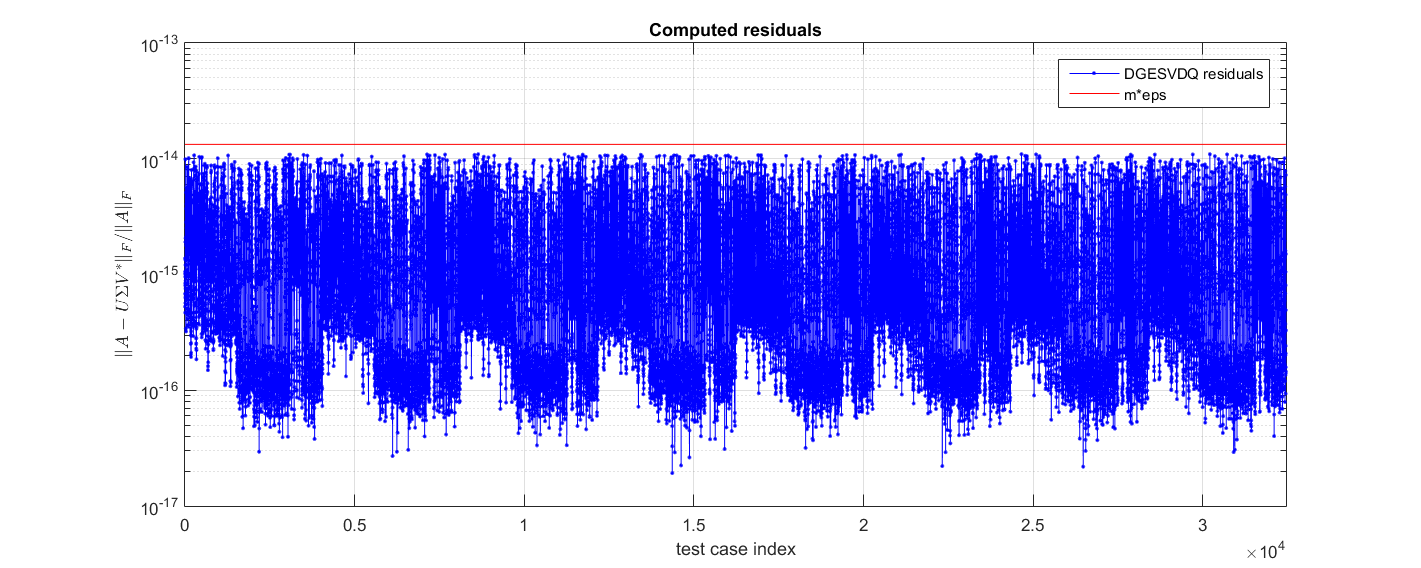
\includegraphics[width=6.3in,height=4.7in]{Fig1.png}
	\end{center}	
	\caption{ \label{fig:1} The residuals $\|A-U\Sigma V^*\|_F / \|A\|_F$.}
\end{figure} 

\begin{figure}[h]
	\begin{center}
		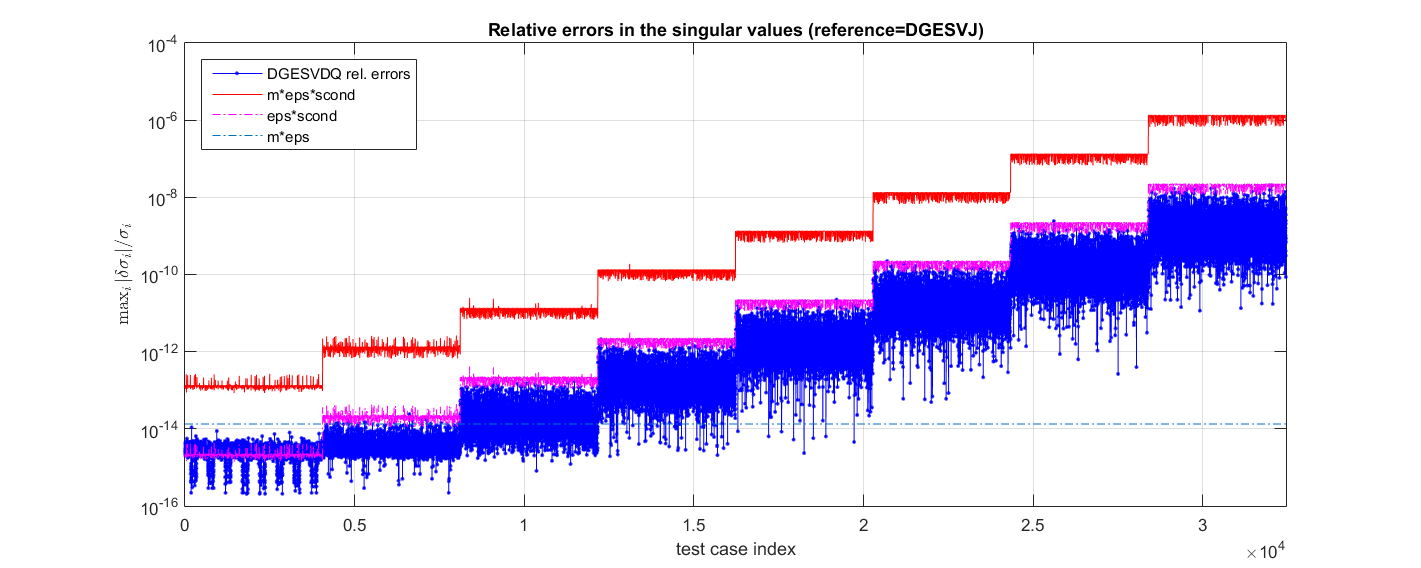
\includegraphics[width=6.3in,height=4.7in]{Fig2.png}
	\end{center}	
	\caption{ \label{fig:2}  Relative errors $\max_i |\delta\sigma_i|/\sigma_i$.}
\end{figure}

\begin{figure}[h]
	\begin{center}
		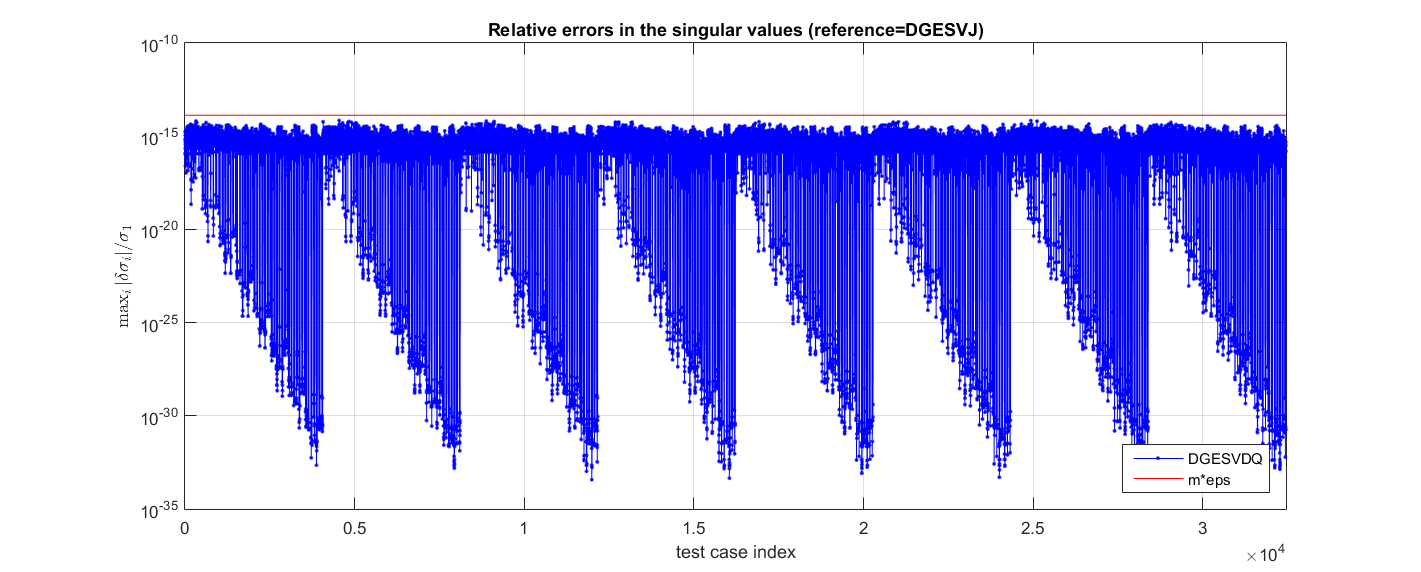
\includegraphics[width=6.3in,height=4.7in]{Fig3.png}
	\end{center}	
	\caption{ \label{fig:3} Relative errors $\max_i |\delta\sigma_i|/\|A\|_2$.}
\end{figure} 

\begin{figure}[h]
	\begin{center}
		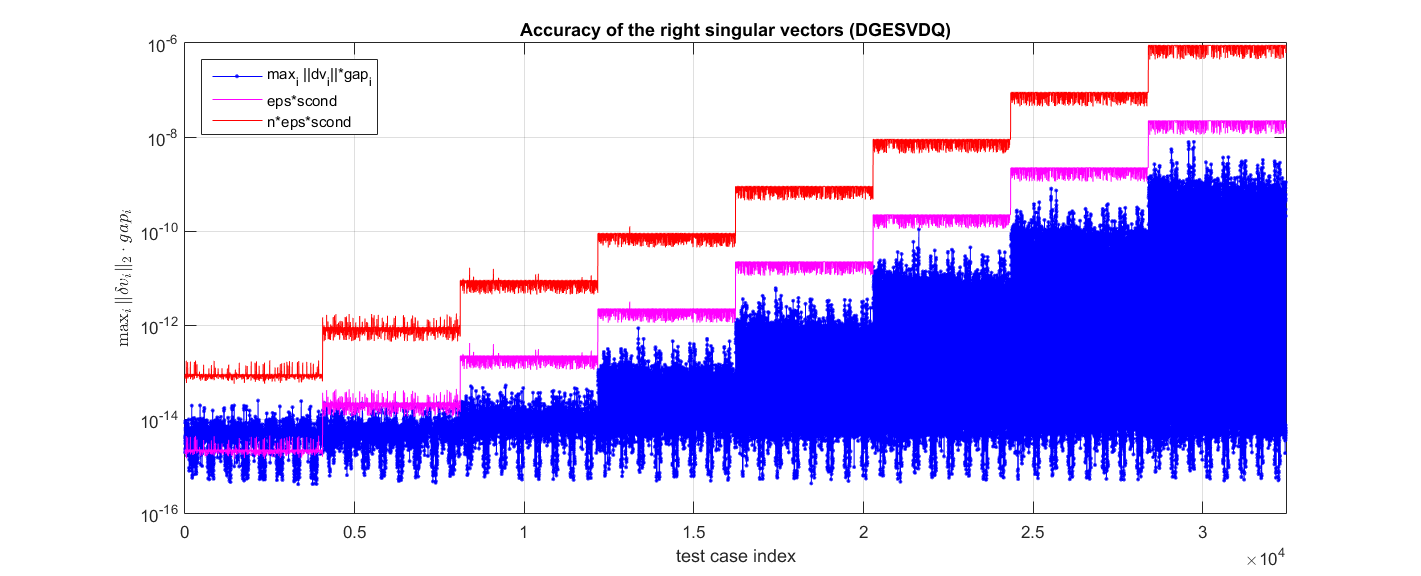
\includegraphics[width=6.3in,height=4.7in]{Fig4.png}
	\end{center}	
	\caption{ \label{fig:4} Accuracy of the computed right singular vectors, compared with the bounds obtained through the perturbation theory.}
\end{figure}

\begin{figure}[h]
	\begin{center}
		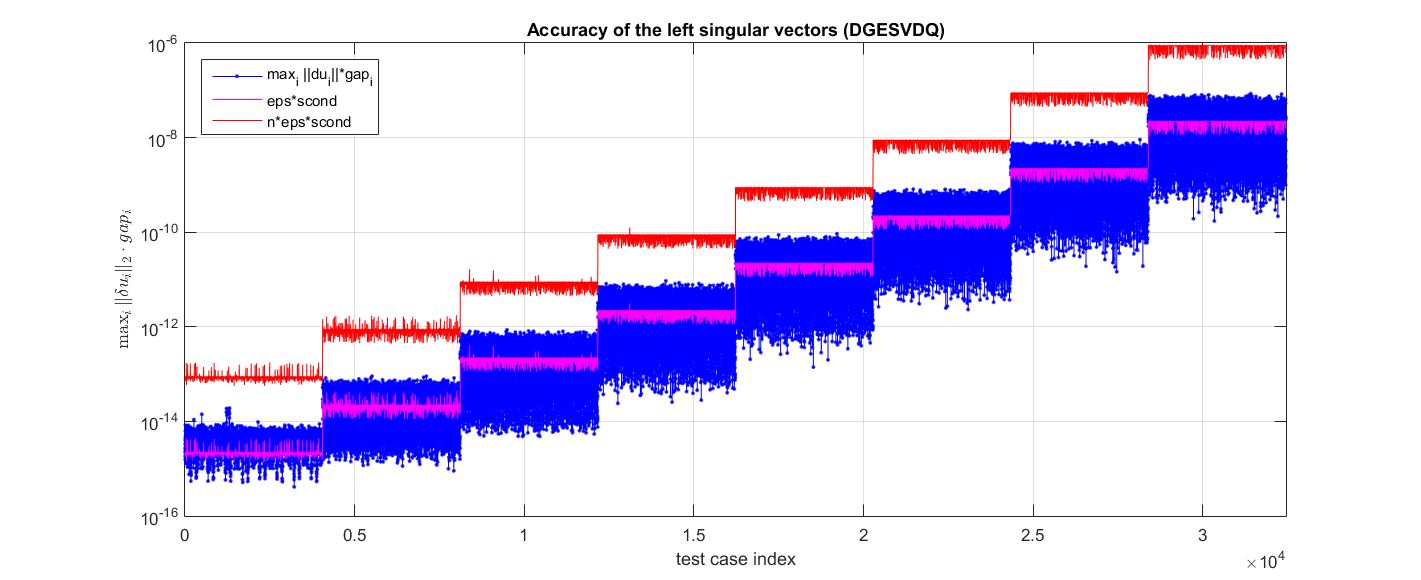
\includegraphics[width=6.3in,height=4.7in]{Fig5.png}
	\end{center}	
	\caption{ \label{fig:5} Accuracy of the computed left singular vectors, compared with the bounds obtained through the perturbation theory.}
\end{figure} 

\begin{figure}[h]
	\begin{center}
		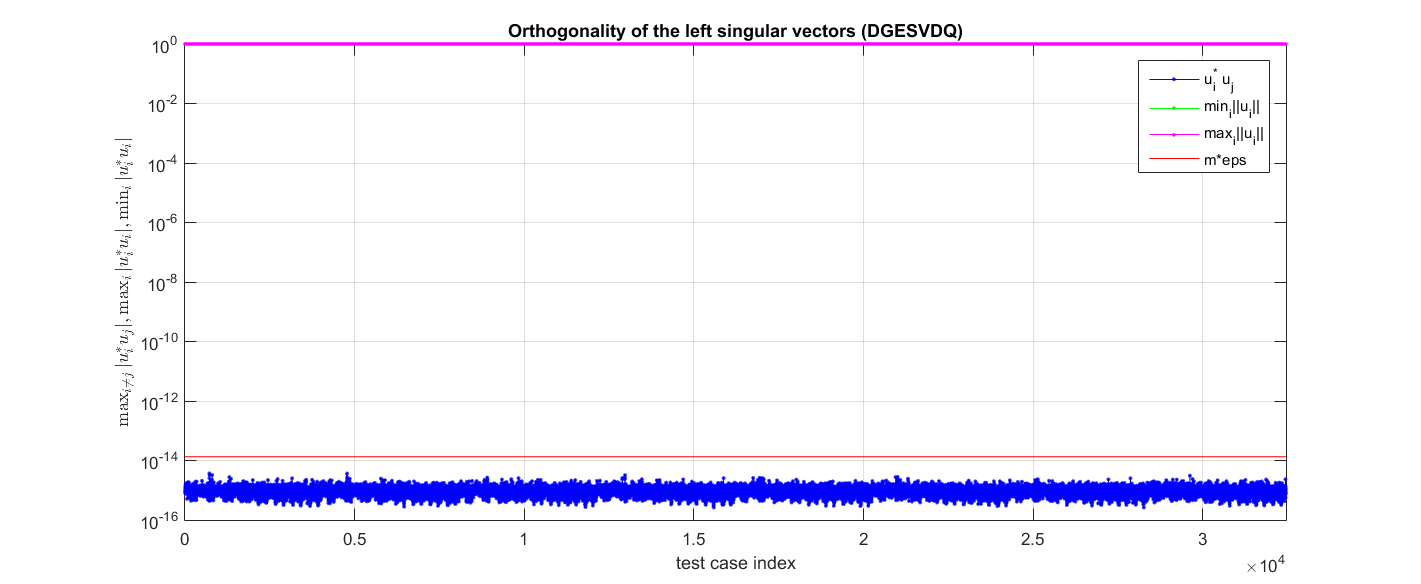
\includegraphics[width=6.3in,height=4.7in]{Fig6.png}
	\end{center}	
	\caption{ \label{fig:6} Orthogonality of the left singular vectors.}
\end{figure}

\begin{figure}[h]
	\begin{center}
		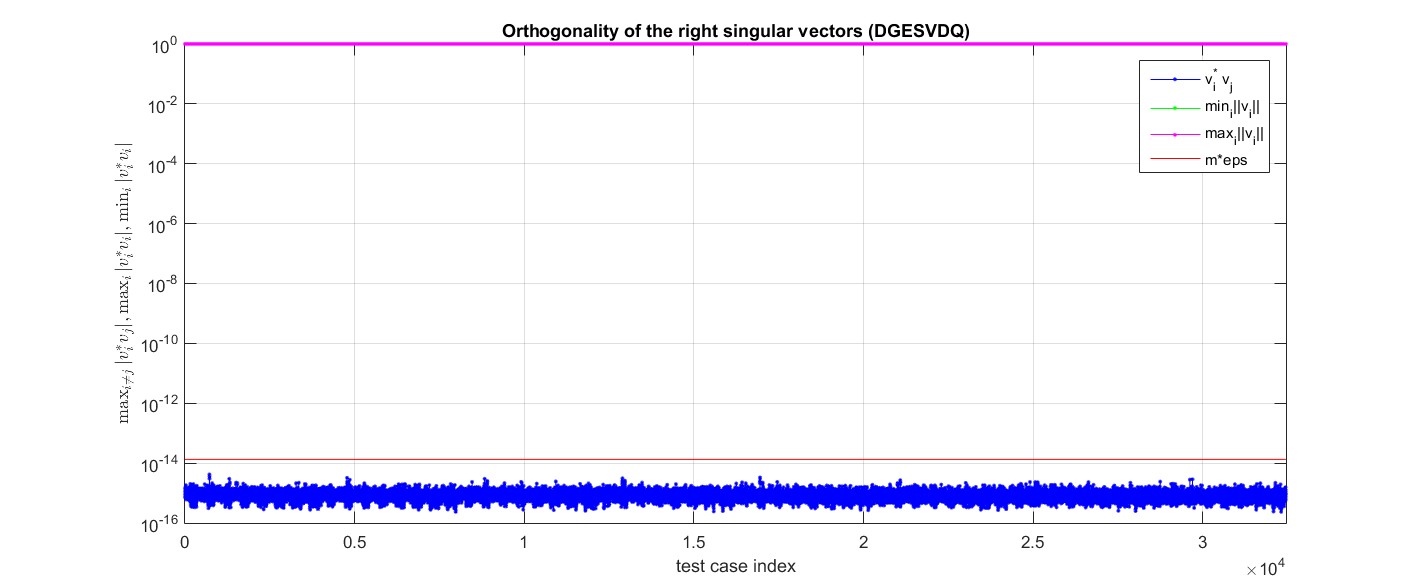
\includegraphics[width=6.3in,height=4.7in]{Fig7.png}
	\end{center}	
	\caption{ \label{fig:7} Orthogonality of the right singular vectors.}
\end{figure} 

\begin{figure}[h]
	\begin{center}
		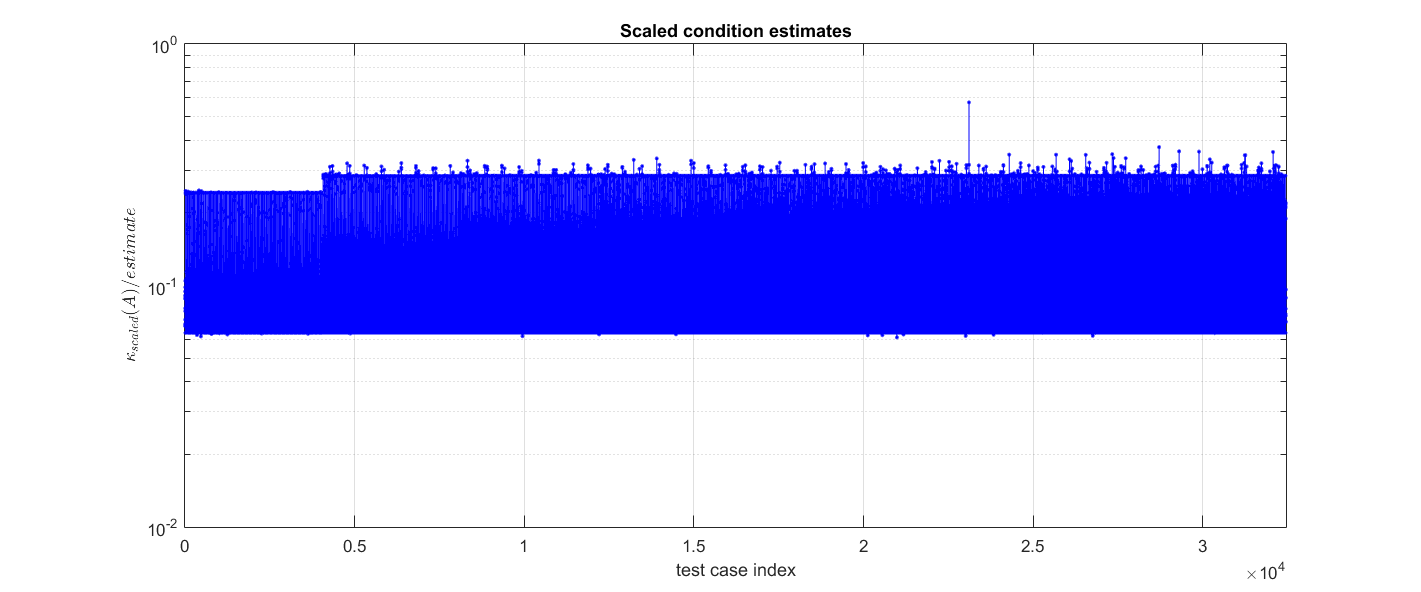
\includegraphics[width=6.3in,height=4.7in]{Fig8.png}
	\end{center}	
	\caption{ \label{fig:8} The quotient of the true (i.e. computed using SVD) and the estimated scaled condition number. }
\end{figure}
\bibliographystyle{plain}
\bibliography{xgesvdq}
\end{document}
